\documentclass[12pt]{article}
\usepackage{geometry}
\usepackage{graphicx}
\usepackage{float}
\usepackage{caption}
\usepackage{subcaption}
\usepackage{booktabs}
\usepackage{amsmath}
\usepackage{hyperref}
\usepackage{siunitx}
\usepackage{tocloft}
\renewcommand{\cftsecfont}{\normalsize} % font size for sections
\renewcommand{\cftsubsecfont}{\small}   % smaller font for subsections
\renewcommand{\cftsecpagefont}{\normalsize} 
\renewcommand{\cftsubsecpagefont}{\small}
\renewcommand{\cftbeforesecskip}{0pt}   % remove extra vertical space
\renewcommand{\cftbeforesubsecskip}{0pt}
\setlength{\cftsecindent}{0pt}
\setlength{\cftsubsecindent}{15pt}

\geometry{margin=1in}
\graphicspath{{figures/}}

\begin{document}

% ------------------ COVER PAGE ------------------
\begin{titlepage}
    \centering
    \vspace*{0.1cm}
    {\huge LUT Characterization \\[0.5em]}
    {\large Fall 2025 \\[2em]}

    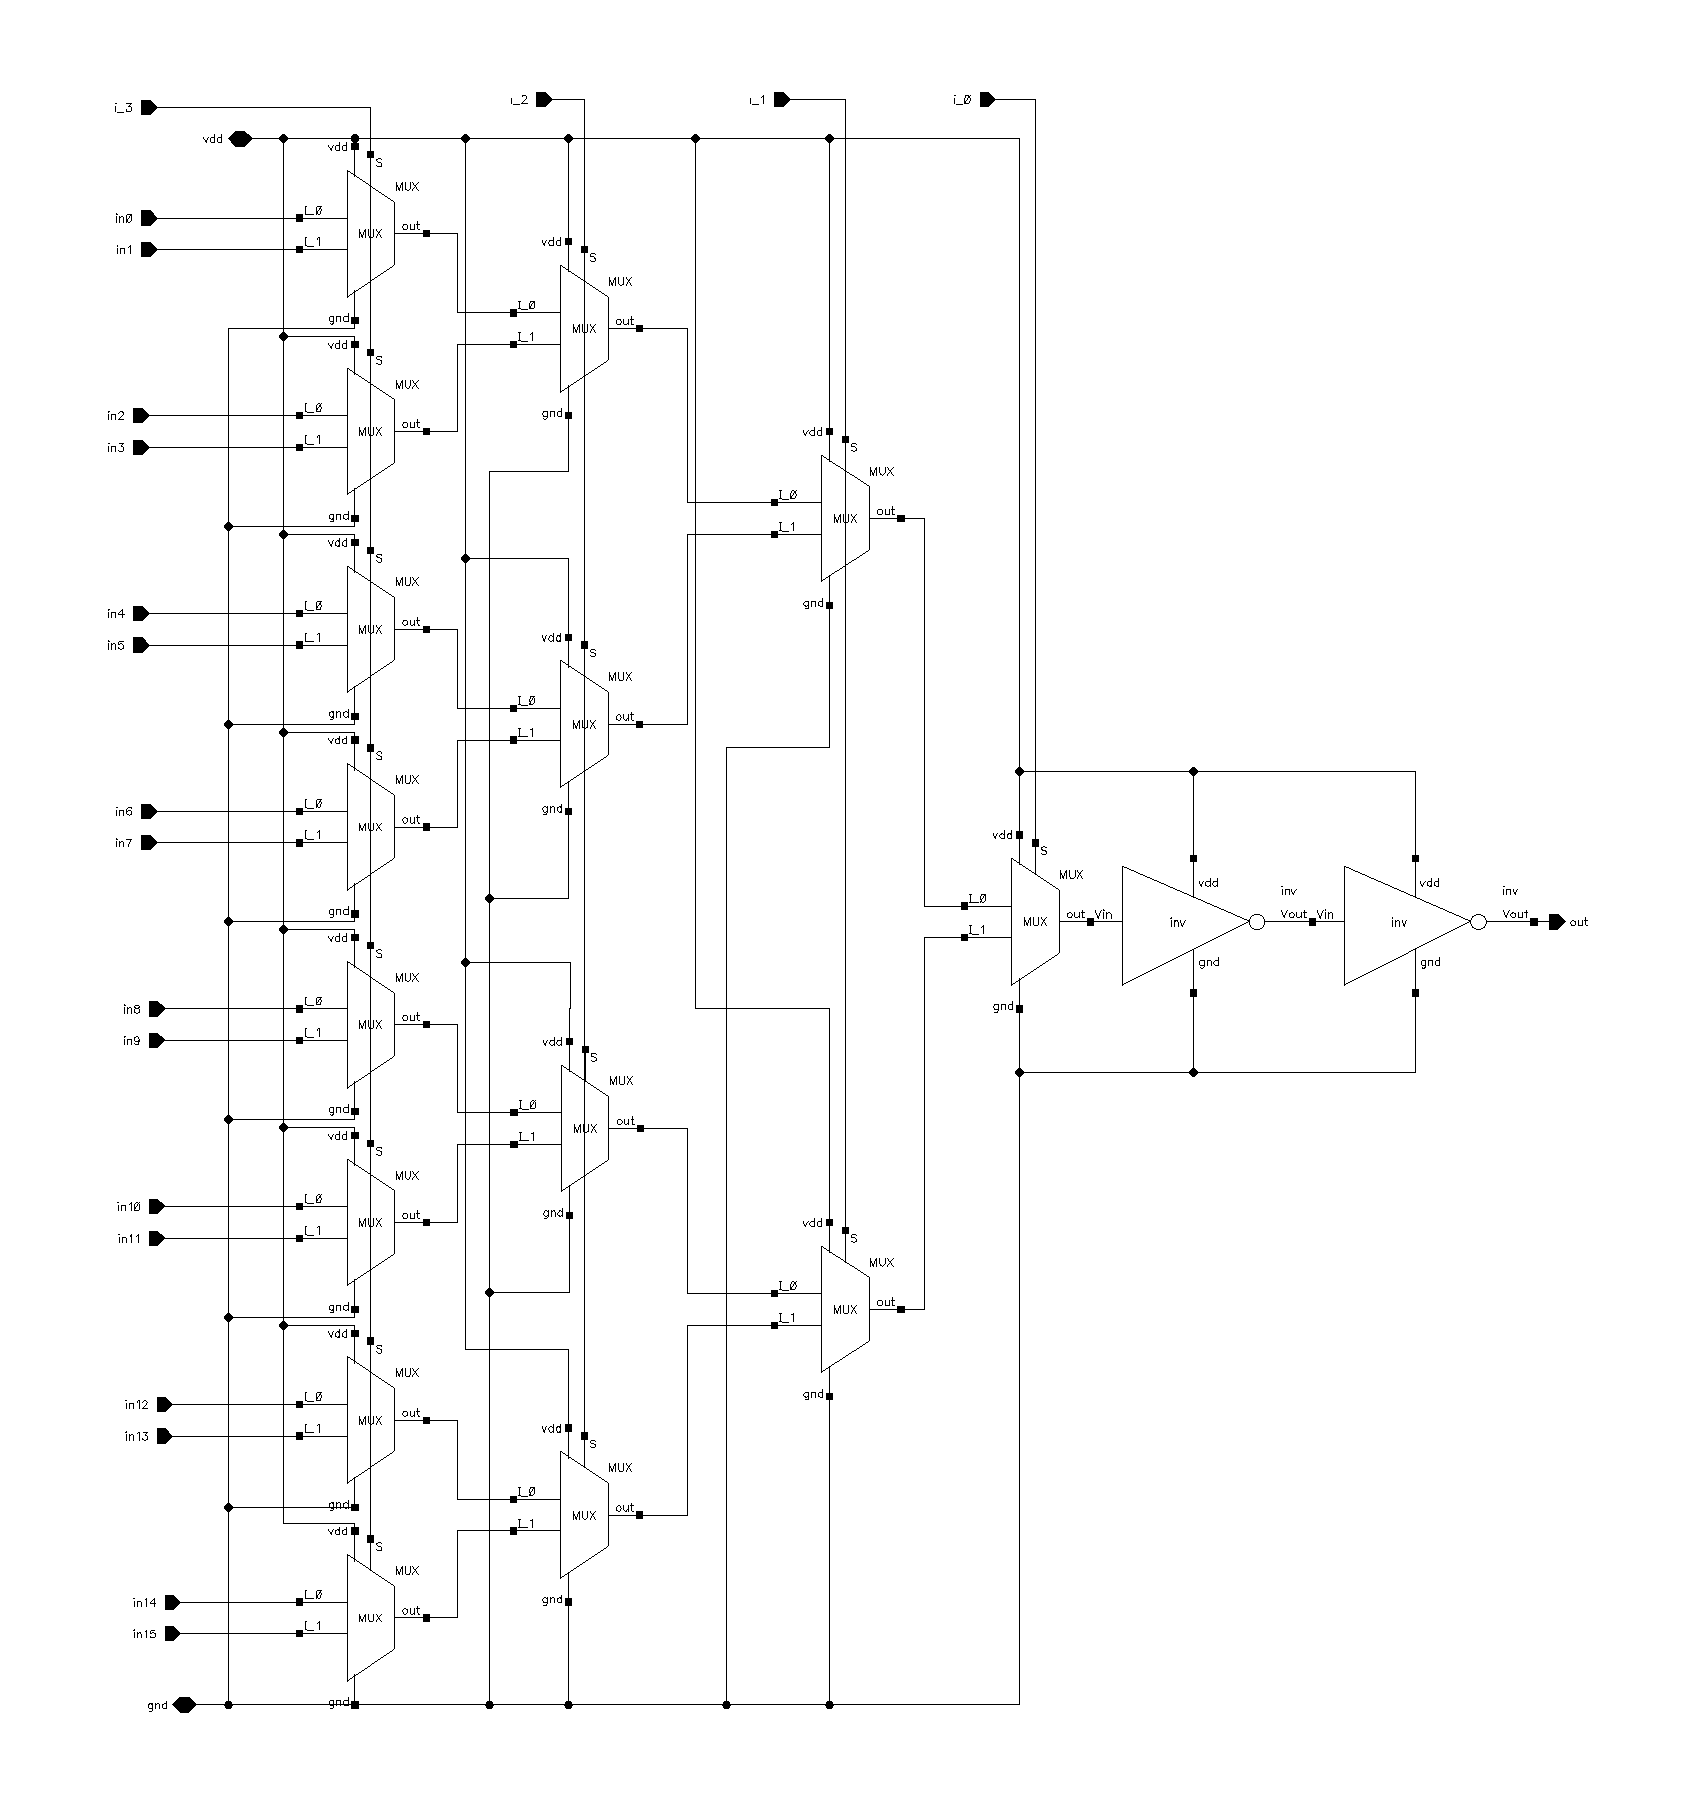
\includegraphics[width=\linewidth]{LUT_sch.png}\\[2em]

    \textbf{Authors:} Krishna Karthikeya Chemudupati, Taarana Jammula \\[2em]

    \vfill
\end{titlepage}

% ------------------ TABLE OF CONTENTS ------------------
\tableofcontents
\newpage

% ------------------ SECTION 1 ------------------
\section{Baseline Design Schematics}

\subsection{Minimum Size Inverter}

\subsubsection*{Schematic}
\begin{figure}[H]
    \centering
    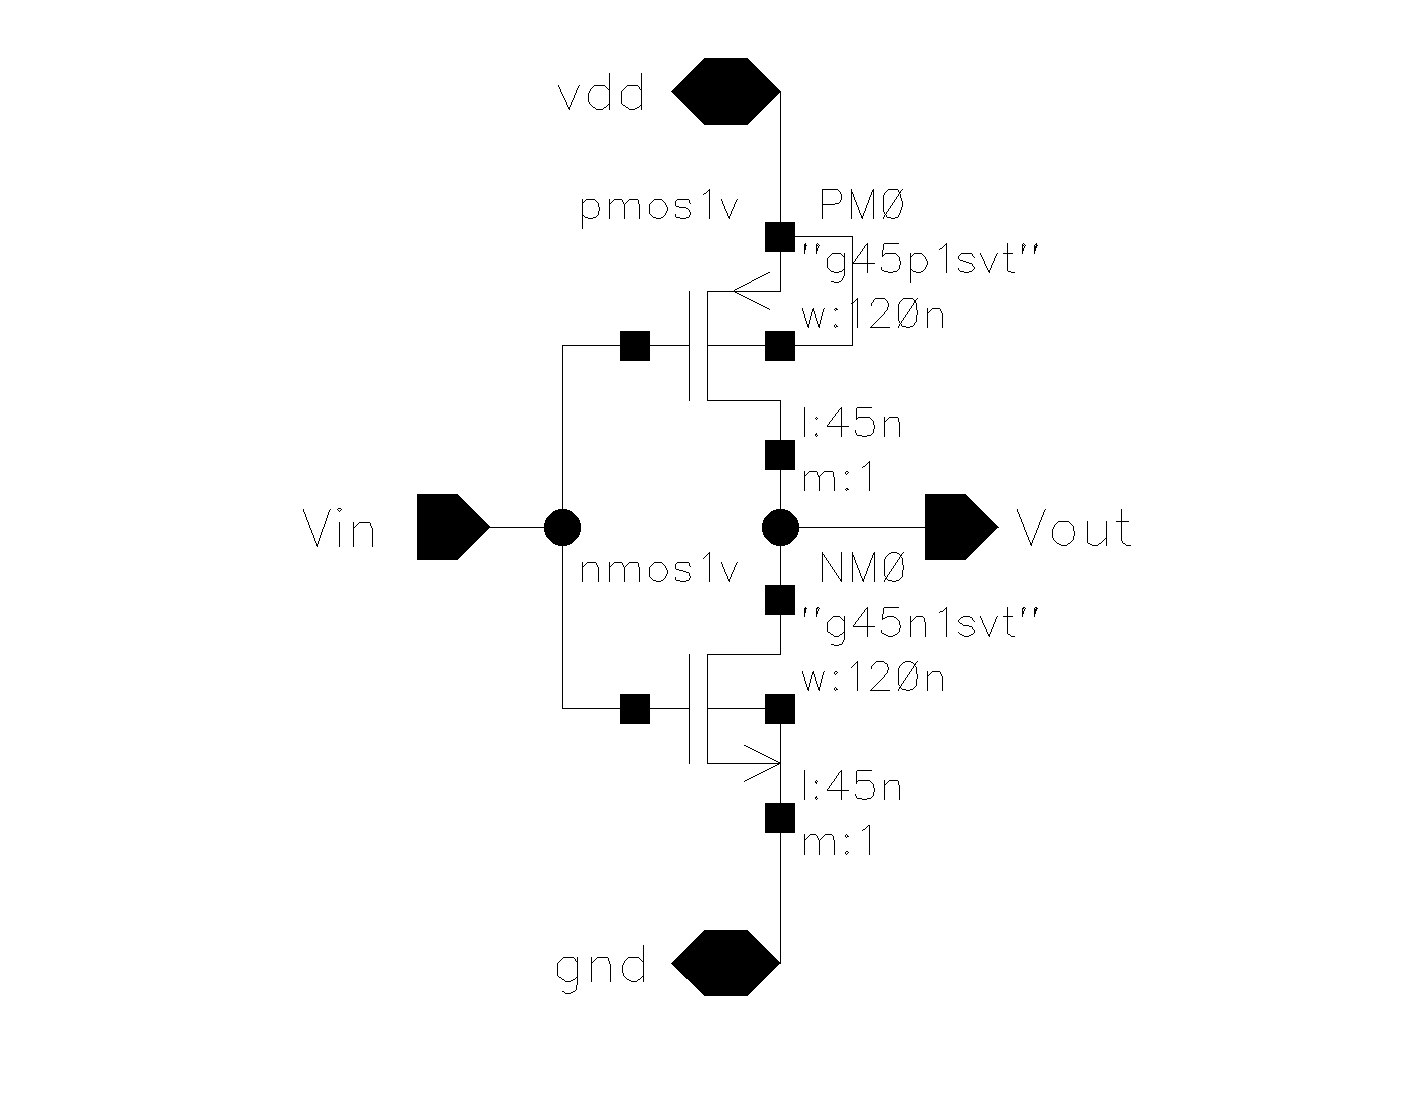
\includegraphics[width=0.5\linewidth]{writeup//figures/inv_sch.png}
    \caption{Enter Caption}
\end{figure}


\subsubsection*{Symbol}
\begin{figure}[H]
    \centering
    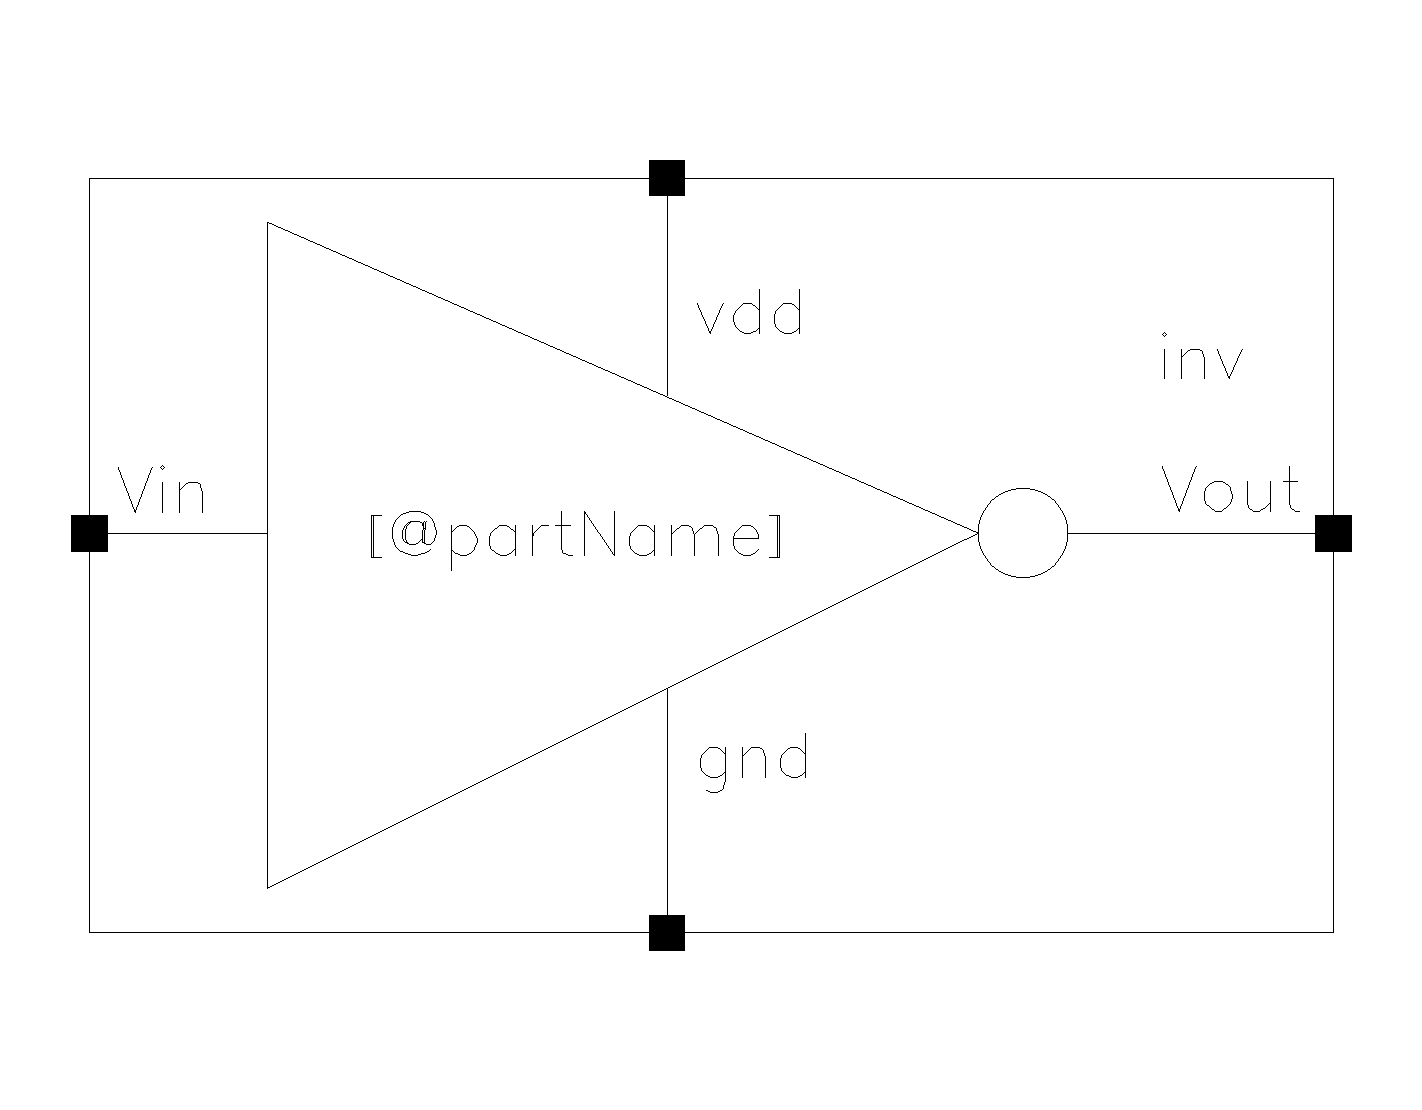
\includegraphics[width=0.5\linewidth]{writeup//figures/inv_sym.png}
    \caption{Enter Caption}
\end{figure}


\newpage

\subsection{2:1 MUX Design}



\newpage

\subsection{16:1 LUT Design}



\newpage

% ------------------ SECTION 2 ------------------
\section{Baseline Design Validation and Logical Test}
\subsection{Test Schematic and Case}
\subsubsection*{2:1 MUX Subcircuit Validation}
\begin{figure}[H]
    \centering
    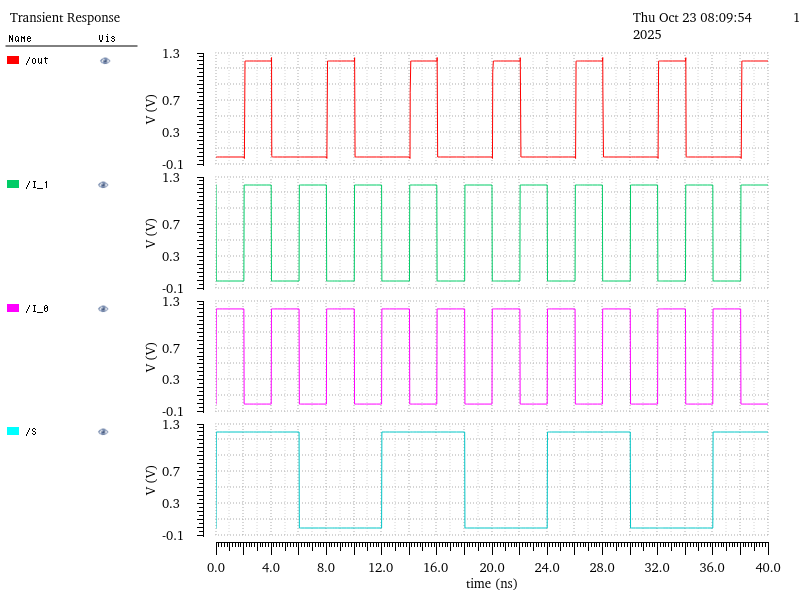
\includegraphics[width=0.5\linewidth]{writeup//figures/muxsubval.png}
    \caption{Enter Caption}
\end{figure}

In the subcircuit test, the select input \( S \) is toggled while \( I_0 \) and \( I_1 \) run as independent square waves. 
Whenever \( S \) is high, the output waveform overlays \( I_1 \) with only a small propagation delay; whenever \( S \) is low, the output overlays \( I_0 \). 
Each handoff can be observed at the transitions of \( S \): during every \( S=1 \) interval the output \( V_{\text{out}} \) matches \( I_1 \), and during every \( S=0 \) interval it matches \( I_0 \). 
This behavior corresponds to the expected logic equation 
\[
V_{\text{out}} = S \cdot I_1 + \overline{S} \cdot I_0
\]
for a 2:1 pass-gate multiplexer. 
The simulation therefore verifies that the subcircuit operates correctly.

\subsubsection*{16:1 LUT Validation}
\begin{figure}[H]
    \centering
    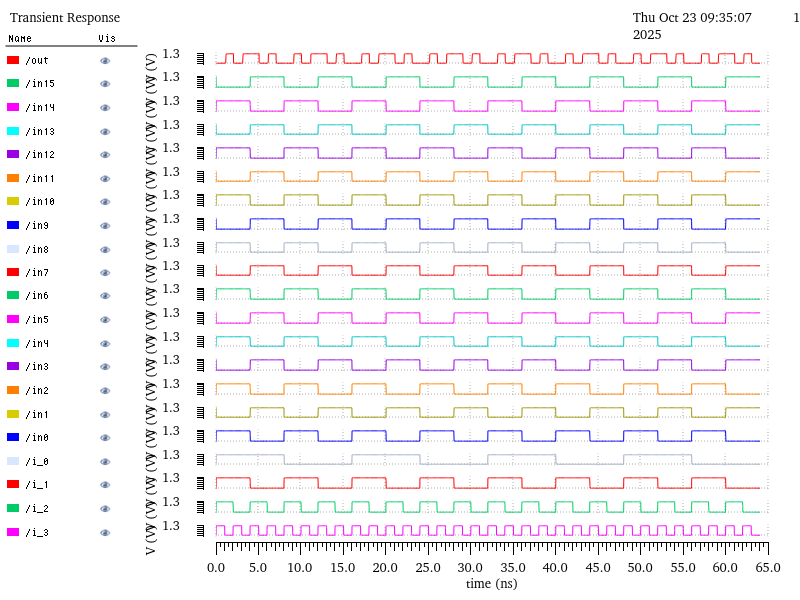
\includegraphics[width=0.5\linewidth]{writeup//figures/lutval.png}
    \caption{Enter Caption}
\end{figure}

For the full 16:1 LUT, all sixteen input combinations (\(2^4\)) were simulated by varying the four address lines from \(0000\) through \(1111\). 
In each address state, the output \(V_{\text{out}}\) aligns with exactly one corresponding data input. 
Specifically, when the address equals \(0000\), \(\text{IN}_0\) propagates to the output; as the address increments, \(\text{IN}_1, \text{IN}_2, \ldots, \text{IN}_{15}\) sequentially drive the output. 
Rising and falling edges on \(V_{\text{out}}\) coincide precisely with the selected input, while nonselected inputs show no coupling. 
Because all address combinations were verified and the output correctly reflected the selected data input each time, the 16:1 LUT simulation confirms correct functionality.


\newpage

\subsection{Simulation Results}
\begin{figure}[H]
    \centering
    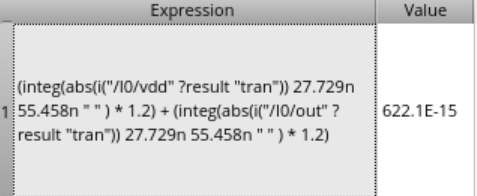
\includegraphics[width=0.5\linewidth]{writeup//figures/baseline_energy_val.png}
    \caption{Enter Caption}
\end{figure}


\newpage

% ------------------ SECTION 3 ------------------
\section{Baseline Delay Measurement}
\subsection{Test Schematic}



\newpage

\subsection{Test Case}



\newpage

\subsection{Simulation Results and Metric Value}
\begin{figure}[H]
    \centering
    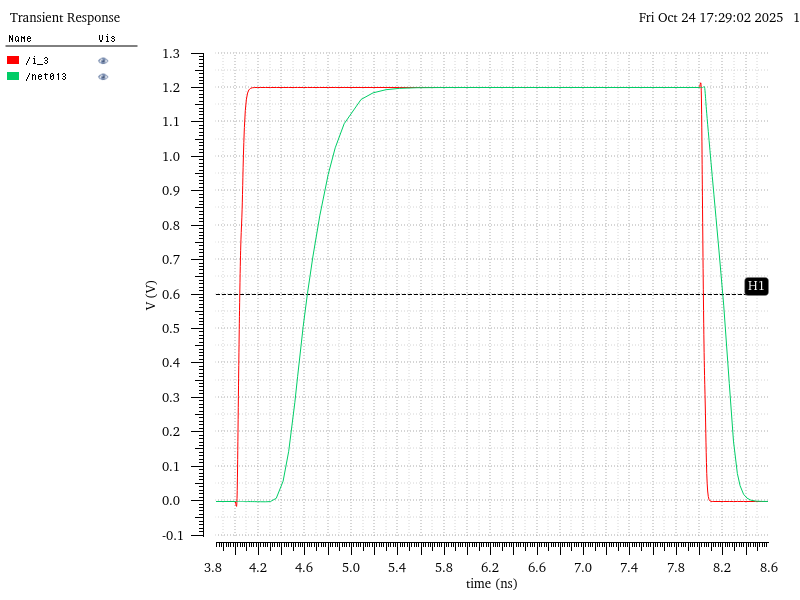
\includegraphics[width=0.5\linewidth]{writeup//figures/baseline_delay_transient.png}
    \caption{Enter Caption}
\end{figure}
Propagation delay measurements are made at the 50\% voltage level of both the input and output signals, which corresponds to \( V = 0.5V_{DD} = 0.6\,\text{V} \) for a 1.2\,V supply.

\subsubsection*{Low-to-High Transition (\(t_{PLH}\))}

For the rising output transition:
\[
t_{PLH} = t_{\text{out,50\%↑}} - t_{\text{in,50\%↓}}
\]
Substituting measured values from the transient response:
\[
t_{PLH} = 4.62003\,\text{ns} - 4.03806\,\text{ns} = 0.58197\,\text{ns}
\]

\subsubsection*{High-to-Low Transition (\(t_{PHL}\))}

For the falling output transition:
\[
t_{PHL} = t_{\text{out,50\%↓}} - t_{\text{in,50\%↑}}
\]
\[
t_{PHL} = 8.19943\,\text{ns} - 8.03239\,\text{ns} = 0.16704\,\text{ns}
\]

\subsubsection*{Average and Worst-Case Delay}

The average propagation delay is given by:
\[
t_p = \frac{t_{PLH} + t_{PHL}}{2}
\]
\[
t_p = \frac{0.58197 + 0.16704}{2} = 0.3745\,\text{ns}
\]

The worst-case delay is the longer of the two:
\[
t_{pd,worst} = \max(t_{PLH}, t_{PHL}) = 0.58197\,\text{ns}
\]

From the results, the rising transition (\(t_{PLH}\)) dominates, indicating that the PMOS network contributes more delay due to its higher effective resistance compared to the NMOS pull-down path. 
Therefore, the \textbf{worst-case propagation delay} of the circuit is approximately \(\mathbf{0.582\,ns}\).


\newpage

% ------------------ SECTION 4 ------------------
\section{Baseline Frequency Measurement}
\subsection{Test Schematic}



\newpage

\subsection{Simulation Results and Metric Value}

\begin{figure}[H]
    \centering
    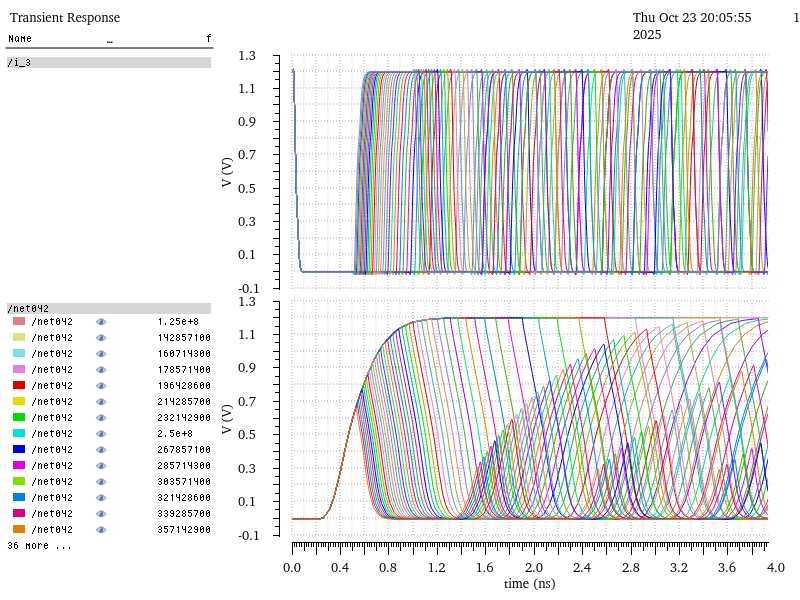
\includegraphics[width=0.75\linewidth]{writeup//figures/frequency_response_param.png}
    \caption{Frequency response at output of the buffer stage}
\end{figure}

\begin{figure}[H]
    \centering
    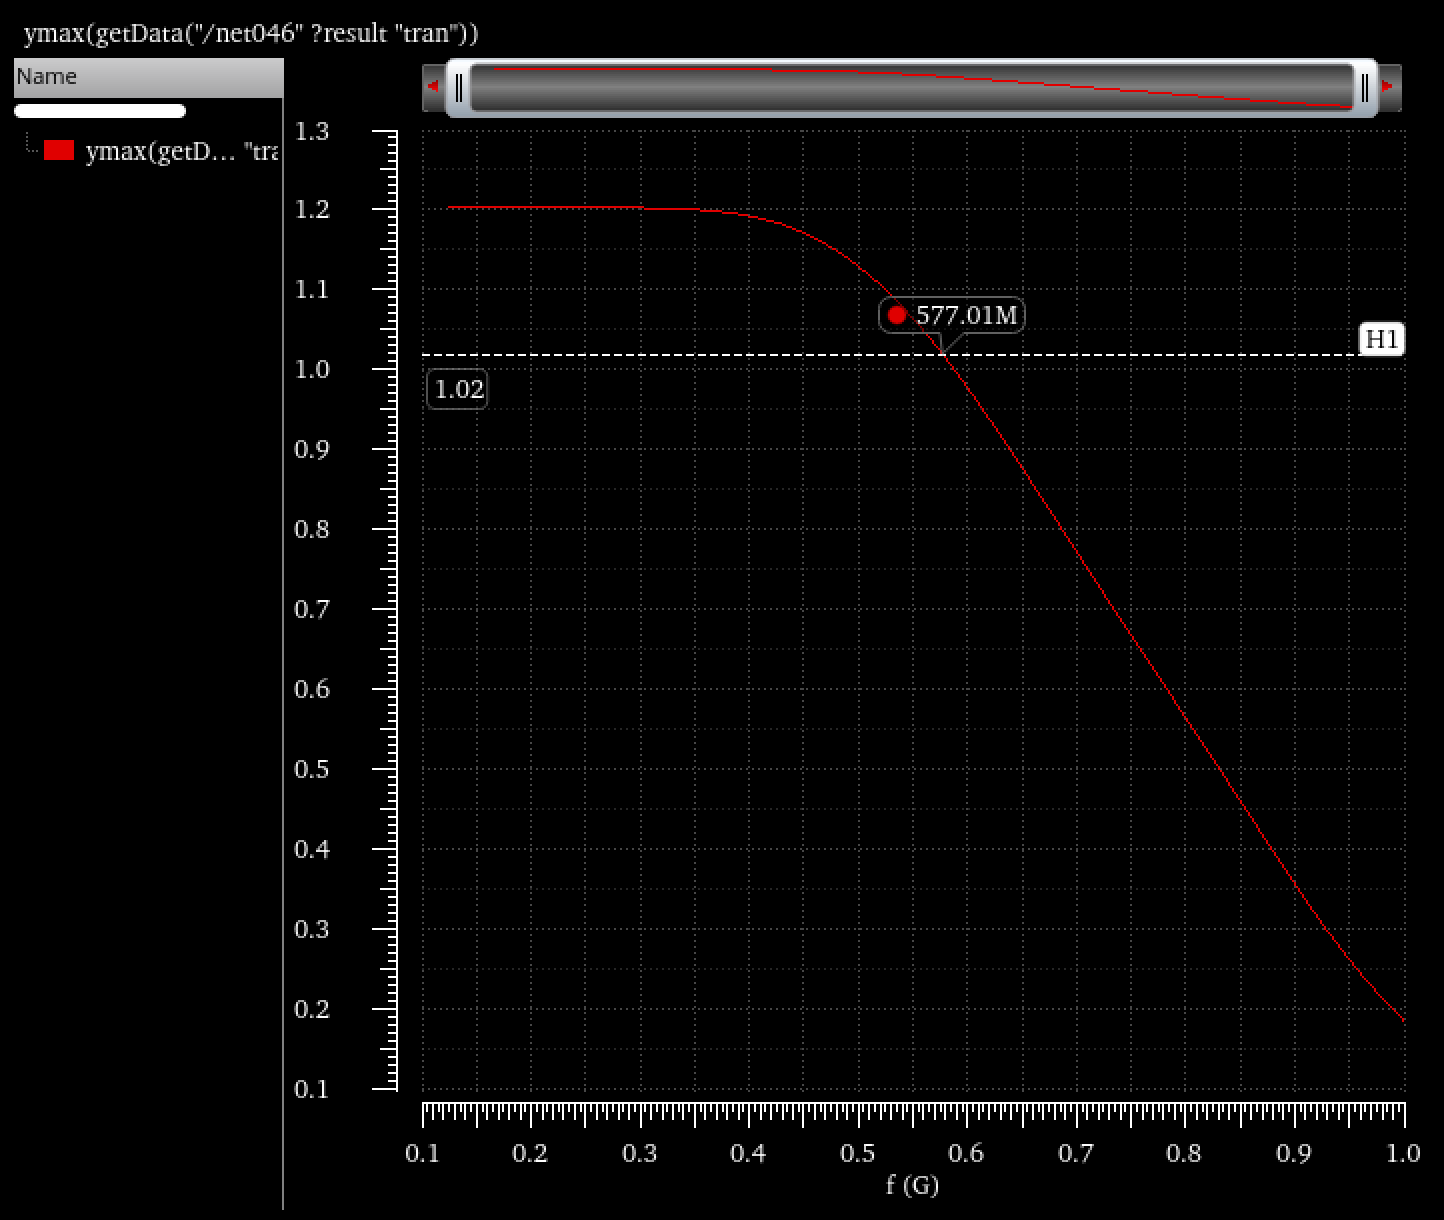
\includegraphics[width=0.75\linewidth]{writeup//figures/max_frequencies.png}
    \caption{Extracting frequency value that allows for 85\% of VDD after buffer stage}
\end{figure}

\newpage

% ------------------ SECTION 5 ------------------
\section{Baseline Energy Measurement}
\subsection{Test Schematic}



\newpage

\subsection{Test Case}



\newpage

\subsection{Simulation Results and Metric Value}
\begin{figure}[H]
    \centering
    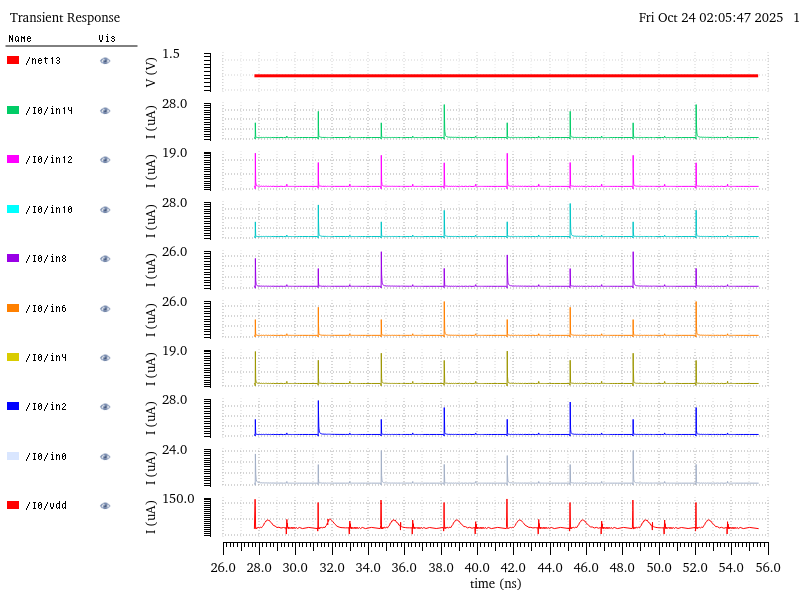
\includegraphics[width=0.5\linewidth]{writeup//figures/baseline_energy_currents.png}
    \caption{Enter Caption}
\end{figure}

\begin{figure}[H]
    \centering
    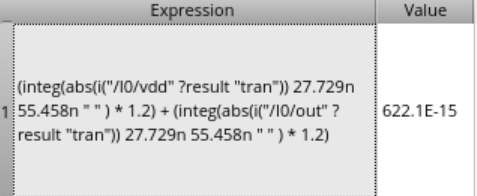
\includegraphics[width=0.5\linewidth]{writeup//figures/baseline_energy_val.png}
    \caption{Enter Caption}
\end{figure}

\newpage

% ------------------ SECTION 6 ------------------
\section{Optimized Design}
\subsection{Optimized Design Schematics}



\newpage

\subsection{Optimization Process}

\begin{figure}[H]
    \centering
    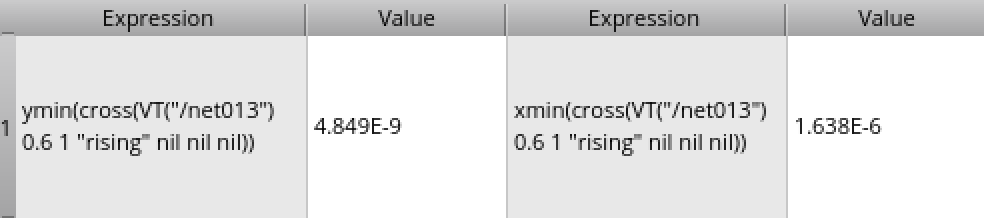
\includegraphics[width=0.5\linewidth]{writeup//figures/optimized_wmux_value.png}
    \caption{Enter Caption}
\end{figure}

\begin{figure}[H]
    \centering
    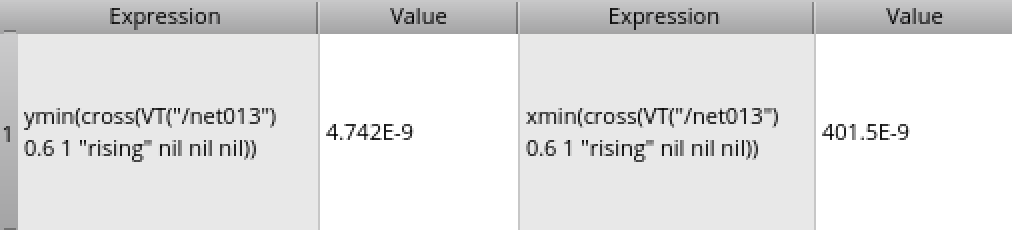
\includegraphics[width=0.5\linewidth]{writeup//figures/optimized_wbuf_value.png}
    \caption{Enter Caption}
\end{figure}

\newpage

% ------------------ SECTION 7 ------------------
\section{Optimized Design Validation and Logical Test}
\subsection{Test Schematic and Case}



\newpage

\subsection{Simulation Results}



\newpage

% ------------------ SECTION 8 ------------------
\section{Optimized Delay Measurement}
\subsection{Test Schematic}



\newpage

\subsection{Test Case}



\newpage

\subsection{Simulation Results and Metric Value}



\newpage

% ------------------ SECTION 9 ------------------
\section{Optimized Frequency Measurement}
\subsection{Test Schematic}



\newpage

\subsection{Simulation Results and Metric Value}



\newpage

% ------------------ SECTION 10 ------------------
\section{Optimized Energy Measurement}
\subsection{Test Schematic}



\newpage

\subsection{Test Case}



\newpage

\subsection{Simulation Results and Metric Value}



\newpage

% ------------------ SECTION 11 ------------------
\section{Comparison Table}



\newpage

% ------------------ SECTION 12 ------------------
\section{Discussion and Conclusions}



\end{document}